\chapter{Basic Examples}\label{chap1}

\section{Introduction}\pageoriginale\label{chap1-sec1.1}

Our aim in these lectures is to study constructive methods for solving
nonlinear systems of the form : 
\begin{equation*}
G(u, \lambda)=0 ,  \tag{1.1}\label{chap1-sec1.1-eq1.1}
\end{equation*}
where $\lambda$ is a possibly multidimensional parameter and $G$ is a
smooth function or operator from a suitable function space into
itself. Frequently we will work in finite dimensional spaces. In this
introductory chapter we present two examples from population dynamics
and study the behaviour of solutions regarding bifurcation, stability
and exchange of stability. Second chapter  describes a local
continuation method and using this we will try to obtain global
solution of \eqref{chap1-sec1.1-eq1.1}. The important tool for
studying this method is 
the \textit{implicit function theorem}. We will also present various
predictor - solver methods. The third chapter deals with global
continuation theory. Degree theory and some of its applications are
presented there. Later in that chapter we will study global homotopies
and Newton methods for obtaining solutions of the equation
\eqref{chap1-sec1.1-eq1.1}.  

In the fourth chapter, we describe a practical procedure for computing
paths and introduce the method of arclength continuation. Using the
bordering   algorithm presented in that chapter, we can compute paths
in an efficient way. In chapter \ref{chap5}, we will study singular points and
bifurcation. A clear description of various methods of continuation
past singular points, folds, branch switching at bifurcations points
is presented\pageoriginale in that chapter. We also study
multiparameter problems, 
Hopfbifurcations later in that chapter. The final chapter presents
some numerical results obtained using some of the techniques presented
in the previous chapters. 


\section{Examples (population dynamics)}\label{chap1-sec1.2}

We start with a simple, but important example from population dynamics
(see \cite{key11}, \cite{key24}). Let $u(t)$ denote the populations
density in a particular region, at time $t$. The simplest growth law
states that the 
\textit{rate of change of population is proportional to the existing
  density, that is:} 
\begin{equation*}
\frac{du}{dt}=\beta u,\tag{1.3}\label{chap1-sec1.2-eq1.3}
\end{equation*}
where $\beta$ is the reproduction rate. The solution for this problem
is given by   
\begin{equation*}
u(t)= u_\circ e^{\beta (t-t_\circ)}, u_\circ = u(t_\circ).
\tag{1.4}\label{chap1-sec1.2-eq1.4} 
\end{equation*}

Note that $u(t)\to \infty$ as $t\to \infty$. This means that
population grows indefinitely with time. Obviously, we know that such
situation is not possible in practice. Hence $\beta$ cannot be a
constant. It must decrease as $u$ increases. Thus as a more realistic
model, we let $\beta$ be a function of $u$, say linear in $u$ : 
\begin{equation*} 
\beta = \beta_1(1-\frac{u}{u_1}). \tag{1.5}\label{chap1-sec1.2-eq1.5}
\end{equation*}

Here $\beta_1 > 0$,  is the ideal reproduction rate, and $u_1$ is the
maximal density that can be supported in the given environment.  
 
Note that if $u > u_1$ then $\beta < 0$ so that $u(t)$ decays. On the
other\pageoriginale hand, if $u < u_1$ then $u(t)$ grows as time increases. The
solutions curve with $\beta$ as above is sketched in
figure \ref{chap1-sec1.2-fig1.1}; it 
is: 
\begin{equation*}
u(t)= \frac{u_\circ u_1e^{\beta_1t}}{(u_1-u_\circ) + u_\circ
  e^{\beta_1 t}},\quad \text{where}\quad u_\circ =
u(0). \tag{1.6}\label{chap1-sec1.2-eq1.6}  
\end{equation*}

\begin{figure}[H]
\centering
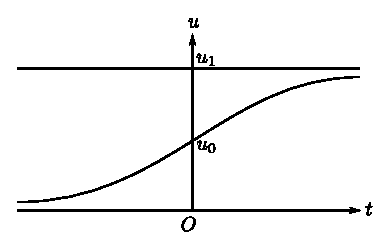
\includegraphics{vol79-fig/fig79-1.eps}
\caption{}
\label{chap1-sec1.2-fig1.1}
\end{figure}


We now consider the more general case, in which coupling with an
external population density, say $u_\circ$, is allowed. Specifically
we take 
\begin{equation*}
\frac{du}{dt}= \beta_1 (1-\frac{u }{u_1})u + \alpha_o (u_\circ
-u)\tag{1.7}\label{chap1-sec1.2-eq1.7} 
\end{equation*}
where, 
\begin{align*}
\beta_1 			&= \text{ ideal reproduction rate} (>0), \\
u_1   	  			&= \text{ maximal density}, \\
u_\circ   			&= \text{ exterior density}, \\
\alpha_\circ   &= \text{ flow rate } (\alpha_\circ \geq 0 \text{ or }
\alpha_\circ \leq 0). 
\end{align*}

Naturally, the population of a particular region may depend upon the
population of the neighbouring regions. If the populations of the
exterior is\pageoriginale less, then species may move to that region
$(\alpha_\circ > 0)$ and vice versa $(\alpha_\circ < 0)$. The term
$\alpha_\circ(u_\circ- u)$ accounts for this behaviour.  

We scale \eqref{chap1-sec1.2-eq1.7} by setting 
\begin{align*}
\lambda_1 & = \frac{\beta_1- \alpha_\circ }{\beta_1}u_1,\\
\lambda_1 & = \frac{\alpha_\circ }{\beta_1}u_1 u_\circ ,\\
t  &= \bar {t}\frac{u_1} {\beta_1}.
\end{align*}

Then we have 
\begin{equation*}
\frac{du}{d\bar{t}} = G(u,\lambda) \equiv -u^2+\lambda_1 u+\lambda_2.
\tag{1.8}\label{chap1-sec1.2-eq1.8} 
\end{equation*}

Here $\lambda = (\lambda_1, \lambda_2)$ denotes the two independent
parameters $\lambda_1$ and $\lambda_2$.  

\medskip
\noindent
\textbf{STEADY STATES}:  The steady state are solutions of 
$$
G(u, \lambda)=0.
$$

These solutions are :
\begin{equation*}
u_\pm = \frac{\lambda_1}{2}+\sqrt{(\frac{\lambda_1}{2})^2+ \lambda_2}
\tag{1.9}\label{chap1-sec1.2-eq1.9} 
\end{equation*}

These solutions are distinct unless
\begin{equation*}
\lambda_2 = -
(\frac{\lambda_1}{2})^2. \tag{1.10}\label{chap1-sec1.2-eq1.10} 
\end{equation*}

Along this curve in the $(\lambda_1, \lambda_2)$ plane, $G_u(u,
\lambda)=0$. This curve is known as a fold (sometimes it is called the
bifurcation set) and the number of solutions changes as one crosses
this curve (See Fig.~\ref{chap1-sec1.2-fig1.2}). 

\begin{figure}[H]
\centering
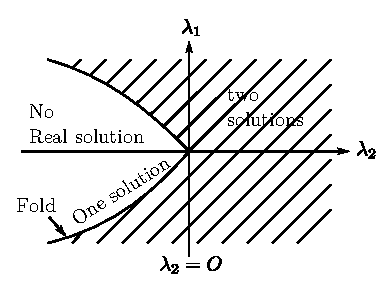
\includegraphics{vol79-fig/fig79-2.eps}
\caption{}
\label{chap1-sec1.2-fig1.2}
\end{figure}\pageoriginale

We examine  three distinct cases : 
$$ 
{\rm (i)} \; \lambda_2 =0 \quad {\rm (ii)} \;  \lambda_2 >0 \quad {\rm
  (iii)} \;  \lambda_2 < 0. 
$$
\begin{enumerate}[(i)]
\item $\lambda_2=0$ : The solutions are two straight lines given by $u
  \equiv 0$ and $u =\lambda_1$. They intersect at the origin. The
  origin is thus a \textbf{bifurcation point}, where two distinct solution
  branches intersect.  

\item $\lambda_2 > 0$ : In this case, there are two solutions $u_+$
  and $u_-$, arcs of the hyperbola, whose asymptotes are given by
  $u=0$ and $u = \lambda_1$.  

\item $\lambda_2 < 0$ : In this case, a real solution exists only if
  $|\lambda_1|>\sqrt{-4\lambda _2}$. They are the hyperbolae conjugate
  to those of case (ii)\break (See Fig.~\ref{chap1-sec1.2-fig1.3}).  
\end{enumerate}

\begin{figure}[H]
\centering
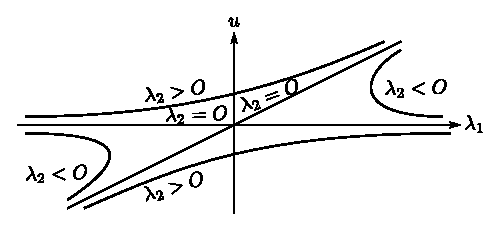
\includegraphics{vol79-fig/fig79-3.eps}
\smallskip
\caption{}
\label{chap1-sec1.2-fig1.3}
\end{figure}

The\pageoriginale solution surfaces in the space $(u, \lambda_1, \lambda_2)$ is
sketched is Fig.~\ref{chap1-sec1.2-fig1.4}. It is clearly a saddle
surface with saddle 
point at the origin. As we see later on, the cases (ii) and (iii)
are example of perturbed bifurcation.  

\begin{figure}[H]
\centering
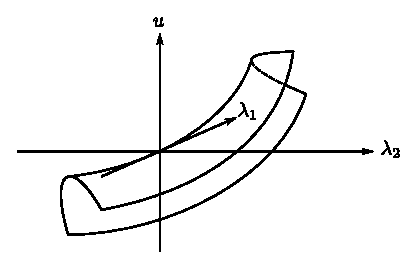
\includegraphics{vol79-fig/fig79-4.eps}
\smallskip
\caption{}
\label{chap1-sec1.2-fig1.4}
\end{figure}

\medskip
\noindent{\textbf{STABILITY}}~: To examine the stability of these
states we note that \eqref{chap1-sec1.2-eq1.8} can be written as: 
\begin{equation*}
\frac{du}{d\bar{t}}= - (u-u_+)(u-u_-).\tag{1.11}\label{chap1-sec1.2-eq1.11}
\end{equation*}

\noindent
Then it clearly follows that :
\begin{equation*}
\frac{du}{d\bar{t}} 
\begin{cases}
<  0  \text{  if  } u < u_- < u_+\\
>  0  \text{  if  } u_- < u < u_+\\
<  0  \text{  if  } u_- < u_+ < u.
\end{cases}\tag{1.12}\label{chap1-sec1.2-eq1.12}
\end{equation*}

This means that $u$ decreases when it is in the semi-infinite
intervals $u < u_-$ and $u_+ < u$. It increases in  $u_- < u <
u_+$. Hence it follows that $u_+$ is always stable and that $u_-$ is
always unstable. Note that the trivial\pageoriginale solution $u
\equiv 0$ consists of 
$u_+$   for  $\lambda_1 < 0$. and $u_-$ for $\lambda_1 > 0$. Thus in
the bifurcation case, $\lambda_2 = 0$, the phenomenon of  exchange of
stability occurs as $\lambda_1$ changes sign. That is the branch which
is stable changes as $\lambda_1$ passes though the bifurcation value
$\lambda_1 = 0$. 

\begin{center}
\begin{minipage}[c]{5cm}
\begin{figure}[H]
\centering
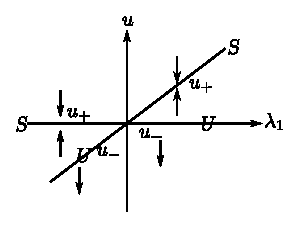
\includegraphics{vol79-fig/fig1.5a.eps}
\caption{$(\lambda_2=0)$}
\label{chap1-sec1.2-fig1.5}
\end{figure}
\end{minipage}
\qquad
\begin{minipage}[c]{5cm}
\begin{figure}[H]
\centering
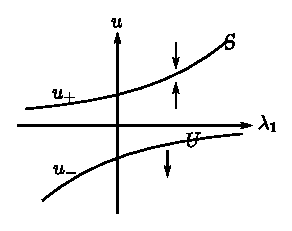
\includegraphics{vol79-fig/fig1.5b.eps}
\caption{$(\lambda_2 > 0)$}
\label{chap1-sec1.2-fig1.6}
\end{figure}
\end{minipage}
\end{center}

%%%
\begin{figure}[H]
\centering
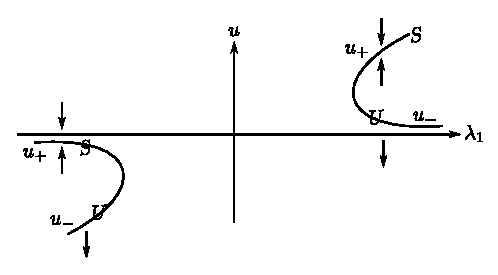
\includegraphics{vol79-fig/fig79-7.eps}
\smallskip
\caption{$(\lambda_2 < 0)$}
\label{chap1-sec1.2-fig1.7}
\end{figure}

We consider another model of reproduction rate $\beta$, say, quadratic
in $u$: 
\begin{equation*}
\beta = \beta_1 [1- (\frac{u}{u_1})^2].\tag {1.13}\label{chap1-sec1.2-eq1.13}
\end{equation*}

Then\pageoriginale equation \eqref{chap1-sec1.2-eq1.8} reduces to : 
\begin{equation*}
\frac{du}{d\bar{t}}= G(u, \lambda) \equiv - u^3 + \lambda_1 u+
\lambda_2, \tag{1.14} \label{chap1-sec1.2-eq1.14} 
\end{equation*}
where now :
\begin{align*}
\lambda_1  & \equiv (1-\frac{\alpha}{\beta_1}) u^2_1, \\
\lambda_2  &\equiv \frac{\alpha}{\beta_1} u_1^2 u_\circ, \\ 
t & \equiv
\bar{t}\frac{u^2_1}{\beta_1}. 
\end{align*}

As before we find steady states and then examine their stability. The study
states are given by the roots of : 
\begin{equation*}
 G(u, \lambda)\equiv - u^3 +\lambda_1 u + \lambda_2 =0
 \tag{1.15}\label{chap1-sec1.2-eq1.15} 
\end{equation*}

The three roots are given by :
\begin{equation*}
u_\circ =a+b, u_\pm \equiv - (\frac{a+b}{2})\pm
i\sqrt{3}(\frac{a-b}{2}) \tag{1.16}\label{chap1-sec1.2-eq1.16} 
\end{equation*}
where, 
\begin{align*}
a &= (\frac{\lambda_2}{2}+ (\frac {\lambda^2 _2}{4}-\frac
{\lambda^3 _1}{27})^{{1/2})^{1/3}}\\ 
b &= (\frac{\lambda_2}{2}+ (\frac {\lambda^2 _2}{4}-\frac{\lambda^3
  _1}{27})^{{1/2})^{1/3}} 
\end{align*}

In particular either we have $3$ real roots or one real root. Clearly,
if $\lambda^2_2 - \dfrac{4}{27}\lambda^3_1> 0 $, the there will one real
root and two conjugate complex roots. If $\lambda_2^2 - \dfrac{4}{27}
\lambda_1^3 = 0$ then there will be three real roots of which two are
equal. If $\lambda^2_2 - \dfrac{4}{27}\lambda^3_1 < 0$ then there will
be three distinct real roots. This can be seen as follows. Put  
$$
a= (a_1 + ib_1)^{1/3}, \text{ then } b =  (a_1 -  ib_1)^{1/3}. 
$$

By changing $a_1 + ib_1$ to polar co-ordinates, we can easily see that
$a+b$ 
is\pageoriginale a real number and $a-b$ is purely imaginary. Now 
$$
G_{u}(u, \lambda) = -3u^{2} + \lambda_{1}.
$$

Combining \eqref{chap1-sec1.2-eq1.15} together with $G_{u}(u, \lambda)
= 0$ we get 
\begin{equation*}
\lambda^{3}_{1} = \frac{27}{4}
\lambda^{2}_{2}.\tag{1.17}\label{chap1-sec1.2-eq1.17} 
\end{equation*}

This curve in the $(\lambda_{1}, \lambda_{2})$ plane represents a \textbf{fold}
where the two real roots become equal; across the fold they become
complex. Again note that across the fold (Bifurcation Set) the number
of solutions changes. Observe that at $\lambda_{2} = 0$, the solution
contains the trivial branch $u = 0$ and the parabola whose branches
are $u_{\pm} = \pm\sqrt{\lambda_{1}}$ which passes through the
origin. Hence the origin is a {\bf{bifurcation point.}} We call this
configuration a {\bf{pitchfork bifurcation.}} For $\lambda_{2} > 0$ or
$\lambda_{2} < 0$ there is no bifurcation. The fold has a cusp at the
origin and is sketched in Fig.~\ref{chap1-sec1.2-fig1.8}.  

\begin{figure}[H]
\centering
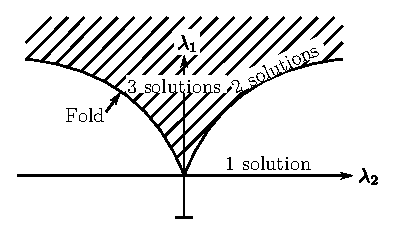
\includegraphics{vol79-fig/fig79-8.eps}
\smallskip
\caption{}
\label{chap1-sec1.2-fig1.8}
\end{figure}

Now we will analyse the stability results in different
cases. \eqref{chap1-sec1.2-eq1.14} can be written as : 
\begin{equation*}
\frac{du}{d \bar{t}} = - (u-u_{o})
(u-u_{+})(u-u_{-}). \tag{1.18}\label{chap1-sec1.2-eq1.18} 
\end{equation*}\pageoriginale
\begin{enumerate}[(i)]
\item $\lambda_{2} = 0$: The dynamic in this case are simply generated
  by,  
\begin{equation*}
\frac{du}{d \bar{t}} = -u(u- \sqrt{\lambda_{1}}) (u +
\sqrt{\lambda_{1}}), \tag{1.19}\label{chap1-sec1.2-eq1.19} 
\end{equation*}
and hence we see that:
\begin{equation*}
\frac{du}{d \bar{t}} \tag{1.20}
\begin{cases}
> 0 ~\text{if} ~ u ~ < - \sqrt{\lambda_{1}} < 0, \\
< 0 ~\text{if} ~ - ~ \sqrt{\lambda_{1}}< u < 0,\\
> 0 ~\text{if} ~ 0 ~ < u < \sqrt{\lambda_{1}}, \\
< 0 ~\text{if} ~ 0 ~ < \sqrt{\lambda_{1}} < u.
\end{cases}\label{chap1-sec1.2-eq1.20}
\end{equation*}

Thus $u_{o}$ is stable for $\lambda_{1} < 0$ and it becomes unstable
as $\lambda_{1}$ changes sign to $\lambda_{1} > 0$. In this latter
range both $u_{\pm}$ are stable. 

\item $\lambda_{2} > 0$: Then
\begin{equation*}
\frac{du}{d \bar{t}} \tag{1.21}
\begin{cases}
> O ~\text{if}~ u < u_{o}, \\
> 0 ~\text{if}~ u_{o} < u < u_{-},\\
> 0 ~\text{if}~ u_{-} < u < u_{+},\\
< 0 ~\text{if}~ u_{+} < u.
\end{cases}\label{chap1-sec1.2-eq1.21}
\end{equation*}

\item $\lambda_{2} < 0$: In a similar way the stability results can be
  obtained here also. 
\end{enumerate}

The stability results are indicated in figures
\ref{chap1-sec1.2-fig1.9}, \ref{chap1-sec1.2-fig1.10},
\ref{chap1-sec1.2-fig1.11}. The 
solution surface is sketched in figure \ref{chap1-sec1.2-fig1.12}.  

\begin{center}
\begin{minipage}[c]{5cm}
\begin{figure}[H]
\centering
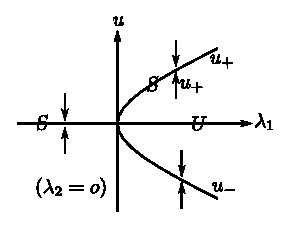
\includegraphics[scale=.95]{vol79-fig/fig1.9.eps}
\smallskip
\caption{$(\lambda_2 =0)$}
\label{chap1-sec1.2-fig1.9}
\end{figure}
\end{minipage}
\qquad
\begin{minipage}[c]{5cm}
\begin{figure}[H]
\centering
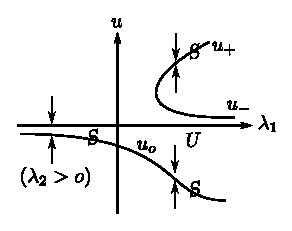
\includegraphics[scale=.95]{vol79-fig/fig1.10.eps}
\smallskip
\caption{$(\lambda_2 > 0)$}
\label{chap1-sec1.2-fig1.10}
\end{figure}
\end{minipage}
\end{center}\pageoriginale

\begin{figure}[H]
\centering 
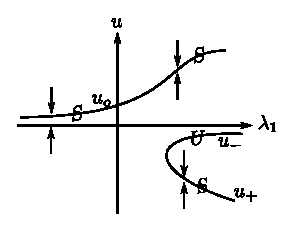
\includegraphics[scale=.95]{vol79-fig/fig79-11.eps}
\smallskip
\caption{$(\lambda_{2}<0)$}
\label{chap1-sec1.2-fig1.11}
\end{figure}

\begin{figure}[H]
\centering 
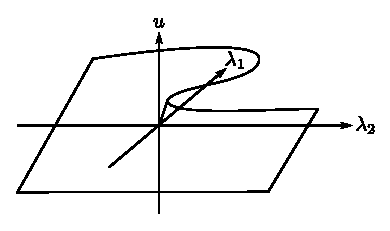
\includegraphics[scale=.95]{vol79-fig/fig79-12.eps}
\smallskip
\caption{}
\label{chap1-sec1.2-fig1.12}
\end{figure}


Now\pageoriginale we present one more example from population dynamics, in which
there are two species in the same region. We know that there is a
constant struggle for survival among different species of animals
living in the same environment. For example, consider a region
inhabited by foxes and rabbits. The foxes eat rabbits and hence this
population grows as the rabbits diminish. But when the population of
rabbits decreases sufficiently the fox population must decrease (due
to hunger). As a result the rabbits are relatively safe and their
population starts to increase again. Thus we can expect a repeated
cycle of increase and decrease of the two species, i.e. a periodic
solution. To model this phenomenon, we take the coupled system :   
\begin{equation*}
\begin{split}
& \tilde{u}_{t} = \beta_{u} [1 - (\frac{\tilde{u}}{\tilde{u}_{1}})^{2} -
  (\frac{\tilde{v}}{\tilde{v}_{1}})^{2}]~ \tilde{u} + \alpha_{u}
(\tilde{u}_{o} - \tilde{u}) - \tilde{\gamma}_{u} \tilde{v},\\ 
& \tilde{v}_{t} = \beta_{v} [1 - (\frac{\tilde{u}}{\tilde{u}_{1}})^{2} -
  (\frac{\tilde{v}}{\tilde{v}_{1}})^{2}]~ \tilde{v} + \alpha_{v}
(\tilde{v}_{o} - \tilde{v}) + \tilde{\gamma}_{v} \tilde{u}.
\end{split}
\tag{1.22} \label{chap1-sec1.2-eq1.22}
\end{equation*}

Here $\tilde{u}$ is prey density and $\tilde{v}$ is predator density
and $\tilde{\gamma}_{u} > 0$, $\tilde{\gamma}_{v} > 0$.  
We have also assumed that both species compete for the same
``vegetation'' so that each of their effective reproduction rates are
diminished together. To scale we now introduce: 
\begin{equation*}
\begin{split}
u & \equiv \frac{\tilde{u}}{\tilde{u}_{1}} ,~ v ~\equiv
\frac{\tilde{v}}{\tilde{v}_{1}},\\
u_{o} & \equiv \frac{\tilde{u}_{o}}{\tilde{u}_{1}} ,~ v_{o} ~\equiv
\frac{\tilde{v}_{o}}{\tilde{v}_{1}}\\  
\gamma_{u} & \equiv  \tilde{\gamma}_{u}
\frac{\tilde{v}_{1}}{\tilde{u}_{1}} ,~ \gamma_{v} ~\equiv
\tilde{\gamma}_{v} \frac{\tilde{u}_{1}}{\tilde{v}_{1}}.  
\end{split}\tag{1.23}\label{chap1-sec1.2-eq1.23}
\end{equation*}

But to simplify we will consider only a special case in which the
eight parameters\pageoriginale  are reduced to one by setting : 
\begin{equation*}
\begin{split}
\beta_{u} & = \beta_{v} = \gamma_{u} = \gamma_{v} = 1,\\
u_{o} & = v_{o} = 0,\\
\lambda & = 1 - \alpha_{u} = 1 - \alpha_{v}. 
 \end{split}\tag{1.24}\label{chap1-sec1.2-eq1.24}
\end{equation*}

 Note that here $\lambda$ is similar to the parameter $\lambda_{1}$ of
 our previous example.  
 
 Now \eqref{chap1-sec1.2-eq1.24} reduces to the system : 
  \begin{equation*}
\binom{u}{v}_{t} = 
\begin{pmatrix}
\lambda & - 1\\ 
1 & \lambda
\end{pmatrix}
 \binom{u}{v} - (u^{2} +
    v^{2}) \binom{u}{v}. \tag{1.25} \label{chap1-sec1.2-eq1.25}
 \end{equation*} 
 
 Note that $\binom{u}{v} = \binom{0}{0}$, the trivial solution is
 valid for all  $\lambda$. First we consider a small perturbation
 $\binom{\delta_u}{\delta_v}$ about the trivial solution
 $\binom{0}{0}$. This 
 satisfies the linearized problem : 
 \begin{equation*}
\binom{\delta_u}{\delta_v}_{t} = A\binom{\delta_u}{\delta_v},
   \text{ \ where \ } A = \begin{pmatrix}\lambda & -1\\  1 &
     \lambda
   \end{pmatrix}. \tag{1.26} \label{chap1-sec1.2-eq1.26} 
 \end{equation*} 

 The eigenvalues of $A$ are given by :
  \begin{equation*}
n_{\pm} = \lambda \pm i. \tag{1.27}\label{chap1-sec1.2-eq1.27}
 \end{equation*} 
 
 These eigenvalues are distinct and hence the solutions of the
 linearized problem must have the form : 
  \begin{equation*}
\begin{split}
 \delta u & = a_{1}e ^{n_{+}t} + a_{2}e ^{n_{-}t} \\
 \delta v & = b_{1}e ^{n_{+}t} + b_{2}e ^{n_{-}t} 
\end{split}\tag{1.28} \label{chap1-sec1.2-eq1.28}
\end{equation*}

For all $\lambda < 0$, we thus have that $\delta u$, $\delta v \to 0$
 as $t \to \infty$. Hence the trivial state is a stable solution. On
 the other hand, if $\lambda > 0$, then $\delta u$, $\delta v$ grow
 exponentially as $t \to \infty$ and the trivial state is unstable for
 $\lambda > 0$.  
  Observe\pageoriginale that there is an exchange of stability as
  $\lambda$ crosses 
 the origin. For $\lambda = 0$ we get periodic solution of the
 linearized problem. Indeed we now show that the exact nonlinear
 solutions have similar feature, but that stable periodic solutions
 exist for all $\lambda > 0$.  
 
 Introduce polar co-ordinates in the $(u,v)$ plane :
\begin{equation*}
 \begin{split}
& u  = \rho \cos \theta , v = \rho \sin \theta,\\ 
& u^{2}+v^{2}   = \rho^{2} , \tan \theta = \frac{v}{u}.
 \end{split}
\tag{1.29} \label{chap1-sec1.2-eq1.29}
\end{equation*}

The system \eqref{chap1-sec1.2-eq1.25} becomes, with $\rho \ge 0$:
\begin{equation*}
\begin{split}
& \dot{\rho} ~\cos ~\theta - \rho \dot{\theta} ~\sin~ \theta = \lambda
\rho ~\cos ~\theta -\rho ~\sin~ \theta - \rho^{3} ~\cos~
\theta,\\ 
& \dot{\rho} ~\sin ~\theta + \rho \dot{\theta} ~\cos~ \theta = \rho
~\cos ~\theta +\lambda\rho ~\sin~ \theta - \rho^{3} ~\cos~ \theta . 
\end{split}
\tag{1.30} \label{chap1-sec1.2-eq1.30}
\end{equation*}

Appropriate combinations of these equations yield : 
\begin{align}
\dot{\rho} &= \lambda\rho - \rho^{3} = \rho(\lambda -
\rho^{2}),\tag{1.31}\label{chap1-sec1.2-eq1.31}\\ 
\dot{\theta} &= +1.\tag{1.32}\label{chap1-sec1.2-eq1.32}  
\end{align}


Thus  $\theta (t) = \theta_0 + t$, where $\theta_{0}$ is an arbitrary
constant. From \eqref{chap1-sec1.2-eq1.31}, for $\lambda > 0$, $\rho
(t)$ is given by $\rho 
(t) (\dfrac{\tau + \rho(t)}{\tau - \rho(t)})^{1/2} = Ce^{\lambda t}$,
where $\tau = \sqrt{\lambda}$ and $C$ is an arbitrary constant. For
$\lambda < 0, \rho (t)$ is given by $\dfrac{\rho(t)}{\sqrt{\rho^{2}(t)
    - \lambda}} = Ce^{\lambda t}$.  We now examine two cases $\lambda
> 0$ and $\lambda < 0$.   
\begin{enumerate}[(i)]
\item $\lambda < 0$: Then $\dot{\rho} < 0$ for all $t$. This implies
  $\rho(t)$ decreases to 0 as $t$ increases.  

\item $\lambda > 0$: Here we have to consider 3 possibilities for
  the state at any\pageoriginale time $t_{o}$:  

(iia)~ $\rho(t_{o}) < \rho_{cr} \equiv \sqrt{\lambda}$

Now~ $\rho(t) < 0$ and $\rho (t)$ increases towards $\rho_{cr}$ as $t
\uparrow \infty$ 

(iib)~$\rho(t_{o}) > \rho_{cr}$

Now~ $\rho(t) < 0$ and $\rho (t)$ decreases towards $\rho_{cr}$ as $t
\uparrow \infty$ 

(iic)~ $\rho(t_{o}) = \rho_{cr}$
\end{enumerate}

Now $\rho(t) \equiv 0 $ and we have the periodic solution :
$$
u = \rho_{cr} ~\cos~ (\theta_{o} + t), v = \rho_{cr} ~\sin~ (\theta_{o} + t).
$$

These solutions are unique upto a phase, $\theta_{o}$. The ``solution
surface'' in the $(u, v, \lambda)$ space contains the trivial branch and
a paraboloid, which is sketched in Fig.~\ref{chap1-sec1.2-fig1.13} 
\begin{figure}[H]
\centering
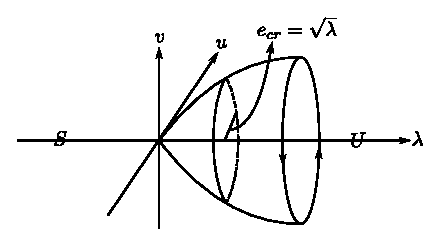
\includegraphics{vol79-fig/fig79-13.eps}
\smallskip
\caption{}
\label{chap1-sec1.2-fig1.13}
\end{figure}

This is a standard example of Hopf bifurcation - a periodic solution
branches off from the trivial steady state as $\lambda$ crosses a
critical value, in this case $\lambda = 0$. The important fact is that
for the complex\pageoriginale pair of eigenvalues $\rho_{\pm}
(\lambda)$, the real 
part crosses zero and as we shall see in general, it is this behaviour
which leads to Hopf bifurcation.  

We have seen the change in the number of solutions across folds and
two types of steady state bifurcations and one type of periodic
bifurcation in our special population dynamics example. We shall now
study much more general steady states and time dependant problems in
which essentially these same phenomena occur. Indeed they are in a
sense typical of the singular behaviour which occurs as parameters are
varied in nonlinear problems. Of course even more varied behaviour is
possible as we shall see (see \cite{key4}, \cite{key13}, \cite{key23},
for example). One 
of the basic tools in studying singular behaviour is to reduce the
abstract case to simple algebraic forms similar to those we have
already studied (or generalizations).    
